% https://www.sharelatex.com/blog/2013/08/27/tikz-series-pt1.html

\documentclass[tikz]{standalone}
\begin{document}
\newcommand{\drawstencil}[2]{%
  \fill[red!30!white] (#1-1,#2) rectangle (#1+2,#2+1);
  \fill[red!30!white] (#1,#2-1) rectangle (#1+1,#2+2);
}
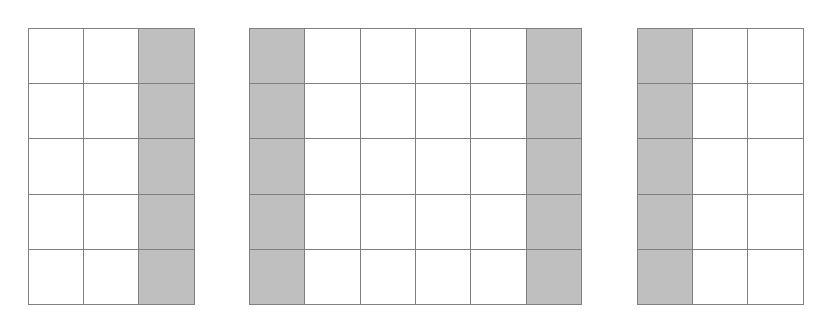
\begin{tikzpicture}[x=2em,y=2em]

  \fill[lightgray](-2,0) rectangle (-1, 5);
  \fill[lightgray] (0,0) rectangle (1,5);
  \fill[lightgray] (5,0) rectangle (6,5);
  \fill[lightgray](7,0) rectangle (8, 5);

  \drawstencil{2}{2}

  \draw[step=1, gray, very thin] (-4,0) grid (-1, 5);
  \draw[step=1, gray, very thin] (0,0) grid (6, 5);
  \draw[step=1, gray, very thin] (7,0) grid (10, 5);

\end{tikzpicture}
\end{document}
